\def\template{../../template/}
\makeatletter \ifx\input@path\@undefined \def\input@path{{\template}} \else \g@addto@macro\input@path{{\template}} \fi \makeatother


% -- Packages --------------------------------------------------------%
\documentclass{rwth-beamer}
\usepackage{diagbox}
\usepackage{pgfplotstable}


% -- Settings --------------------------------------------------------%
\definecolor{mycolor}{HTML}{D1CBF2} % pink


% -- Title --------------------------------------------------------%
\title{Optimales Lager\enspace|\enspace JTL Software GmbH}
\author{Jaro, Martin, Veronika, Lisette, Henning, Daniel und Clemens}
% HINWEIS:  Alphabetisch nach Nachnamen sortieren
%\titlegraphic{
\includegraphics[trim=60pt 95pt 60pt 95pt, clip, height=2em]{logo/cammp}}
\titlegraphic{
\includegraphics[height=2em]{logo/nurcammp}}
\date{Aachen, 19. Juni 2023}
\backgroundgraphic{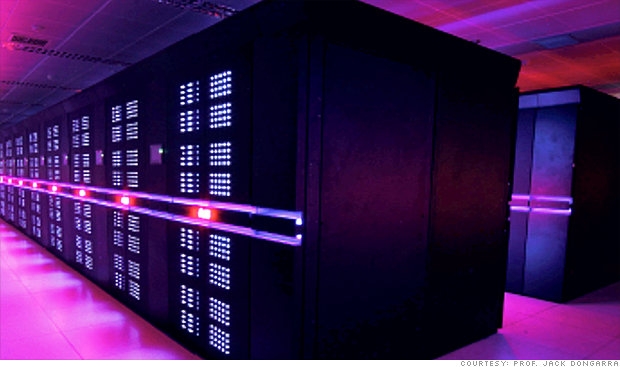
\includegraphics[trim=0pt 0pt 0pt 0pt, clip, width=\paperwidth]{../figs/z_supercomputer}}
\footline{Clemens, Daniel, Jaro, Henning, Lisette, Martin, Veronika\enspace|\enspace\inserttitle}


%----------------------------------------------------------%
\begin{document}

% Title page
\maketitle

% Outline
\begin{frame}
	\frametitle{Outline}
	\tableofcontents
\end{frame}


%----------------------------------------------------------%
\begin{frame}[t]  % t=top,  c=centriert,  b=bottom
	\frametitle{Bilder einfügen}
	\begin{center}
		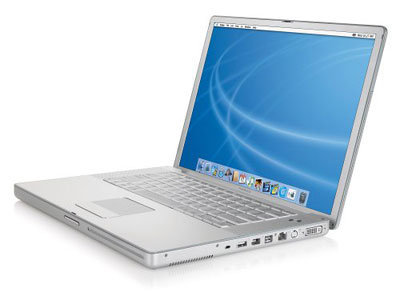
\includegraphics[width=0.7\textwidth]{../figs/z_laptop}
	\end{center}
\end{frame}

\begin{frame}[t]
	\frametitle{Bilder hintereinander einfügen}
	\begin{center}
		\uncover<1->{ 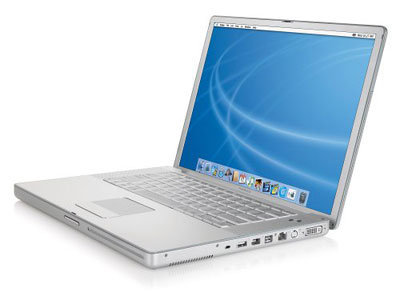
\includegraphics[width=0.3\textwidth]{../figs/z_laptop} }
		\uncover<2-3>{ 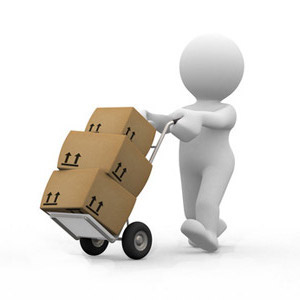
\includegraphics[width=0.3\textwidth]{../figs/z_lieferant} }
		\uncover<3-4>{ 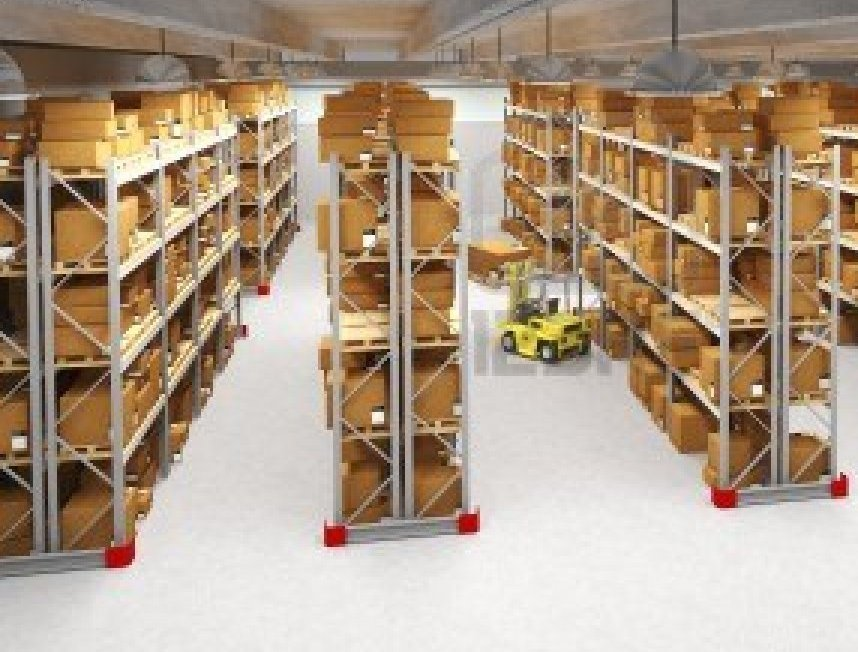
\includegraphics[width=0.3\textwidth]{../figs/z_lager} }
	\end{center}
\end{frame}

%----------------------------------------------------------%
\begin{frame}[t]
	\frametitle{Textformatierung}
	
	Text {\bf fett} schreiben. \\
	Text {\it kursiv} schreiben. \\
	Text \underline{unterstrichen} schreiben. \\
	Text {\color{red} rot}, {\color{blue} blau},  {\color{darkgreen} grün}, {\color{gray} grau},  {\color{blue!60!red} etc.}  schreiben. \\
	Text {\small klein} und {\footnotesize kleiner} schreiben. \\
	Text {\large groß} und {\Large größer} schreiben. \\
	
	\begin{block}{Wichtigen Text in einem Block darstellen}
		Hier wichtiger Text \\
		beispielsweise eine wichtige Formel \\
		oder eine wichtige Beobachtung
	\end{block}
\end{frame}


%----------------------------------------------------------%
\begin{frame}[t]
	\frametitle{Formeln}
	
	{\bf Formeln schreiben} \\
	Ungefähr $\approx$, Multiplikation $\cdot$, Brüche $\frac{20}{21}$, \\
	Pfeile $\rightarrow, \Rightarrow, \leftarrow, \Leftarrow, \leftrightarrow, \Leftrightarrow$, \\
	Sinus $\sin(x)$, Cosinus $\cos(x)$, Integral $\int_a^b f(x) dx$,
	\\[5mm]
	{\bf Formel}
	$$
		\int_{a}^{b} f(x) dx = \int_{a}^{b} \sin(x) \cdot \cos(x) \cdot \frac{20}{3} dx
	$$
	{\bf Formel aus Wikipedia kopieren}\\
	Gehe z.B. auf	\url{http://de.wikipedia.org/wiki/Binomialkoeffizient}
	Markiere dort eine Formel (Bild), kopiere sie mit \, \tt{Cmd + C} \, und füge sie in das Dokument ein mit \, \tt{Cmd + V}.
	Beachte, dass um die Formel noch die \$ Zeichen oder Doppel-\$ Zeichen stehen müssen.
\end{frame}



%----------------------------------------------------------%
\begin{frame}[t]
\frametitle{Aufzählungen}
	Durchnumerierte Aufzählungen
	\large
	\begin{enumerate}
		\item<1-> Ausgangssituation: 
		\item<2-> Statistik überArtikel
		\item<3-> Ziel: Bestmögliche Einsortierung in Warenlager
	\end{enumerate}
	%
	\vspace*{1cm}
	%
	Aufzählungen
	\begin{itemize}
		\item<4-> leeres Lager
		\item<5-6> Einkaufslisten {\color{red} (verschwindet nach zwei Unterfolien)}
		\item<6-> Statistik über Artikel
		\item<6-> Kaufhäufigkeit
		\item<7-> Kombinationskäufe
		\item<8-> Auswertung
	\end{itemize}						
\end{frame}



%----------------------------------------------------------%
\begin{frame}
\frametitle{Einfache Zeichnungen in LaTeX}
	\begin{center}
	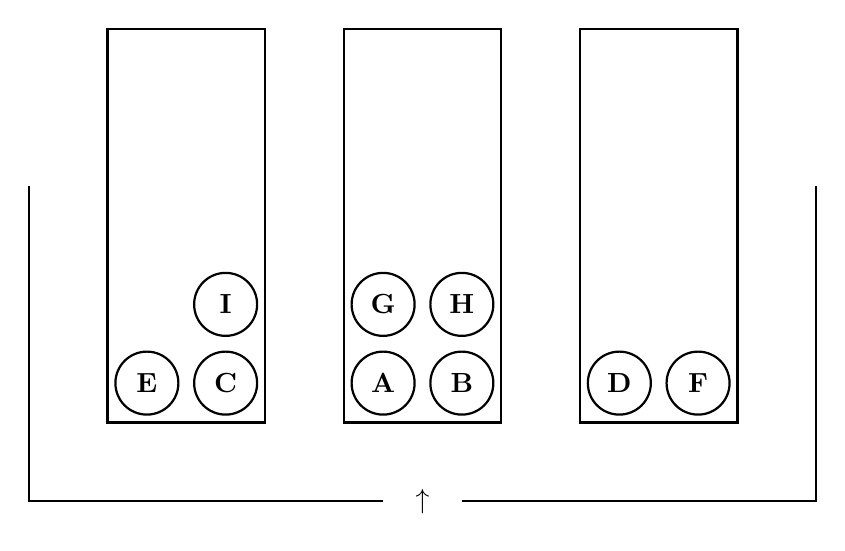
\begin{tikzpicture}
		\draw[thick] (0,4) |- (4.5,0);
		\draw[thick] (5.5,0) -| (10,4);
		\node at (5,0){$\uparrow$};
		%
		\draw[thick] (1,1) rectangle (3,6);
		\draw[thick] (4,1) rectangle (6,6);
		\draw[thick] (7,1) rectangle (9,6);
		%
		\uncover<2->{
			\draw[thick] (1.5,1.5) circle(0.4cm) node {\bf E};
			\draw[thick] (2.5,1.5) circle(0.4cm) node {\bf C};
			\draw[thick] (4.5,1.5) circle(0.4cm) node {\bf A};
			\draw[thick] (5.5,1.5) circle(0.4cm) node {\bf B};
			\draw[thick] (7.5,1.5) circle(0.4cm) node {\bf D};
			\draw[thick] (8.5,1.5) circle(0.4cm) node {\bf F};
			\draw[thick] (2.5,2.5) circle(0.4cm) node {\bf I};
			\draw[thick] (4.5,2.5) circle(0.4cm) node {\bf G};
			\draw[thick] (5.5,2.5) circle(0.4cm) node {\bf H};
		}%
	\end{tikzpicture}
	\\%
	\only<1>{Ein Lager}%
	\only<2>{Artikel einsortieren}%
	\end{center}
\end{frame}



%----------------------------------------------------------%
\begin{frame}
	\frametitle{Datendiagramme}
	\centering
	\begin{minipage}{.45\textwidth}
	Quoten:\\
		\begin{tabular}{|c|c|}
			\hline
			Spedition & Quoten\\
			\hline
			\hline
			1 & 20\% \\
			\hline
			2 & 30\% \\
			\hline
			3 & 50\% \\
			\hline
		\end{tabular}
	\end{minipage}
	\pause
	\hfill
	\begin{minipage}{.45\textwidth}
	Quoten:\\
		\begin{tabular}{|c|c|}
			\hline
			Spedition & Quoten\\
			\hline
			\hline
			1 & 20\% \\
			\hline
			2 & 30\% \\
			\hline
			3 & 50\% \\
			\hline
		\end{tabular}
	\end{minipage}\\[1ex]
	\pause
	\begin{minipage}{\textwidth}
	\begin{center}
	Kapazit\"aten
	\end{center}
		\begin{tabular}[c]{|c||c|c|c|}
			\hline
			\diagbox{LKW-Klasse}{Speditionen} & Spedition 1	& Spedition 2	&Spedition 3\\
			\hline
			\hline
			1 & 2 & 2 & 3\\
			\hline
			2 & 0 & 1 & 2\\
			\hline
		\end{tabular}
	\end{minipage}
\end{frame}



%----------------------------------------------------------%
\begin{frame}
	\frametitle{Flußdiagramm}
	\centering
	\resizebox{!}{(\paperheight)/2}{
			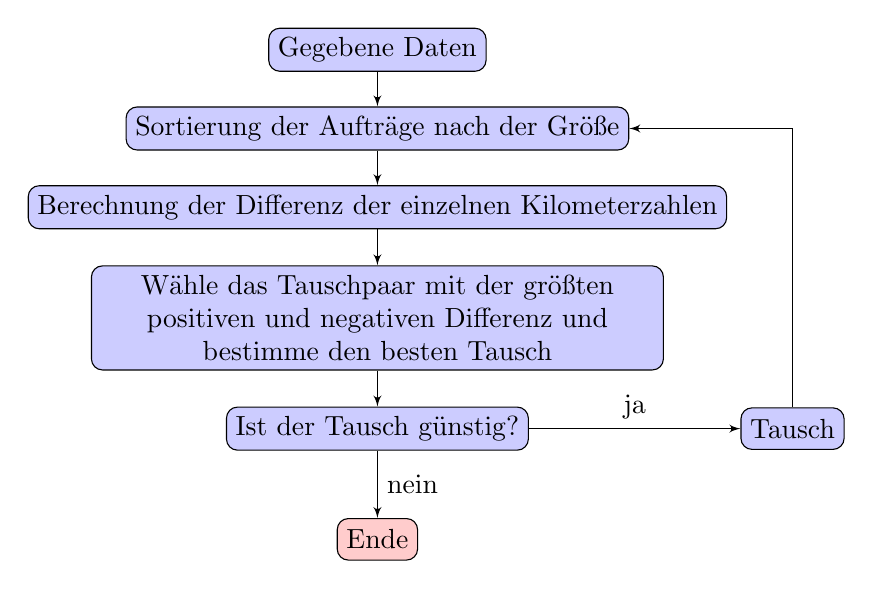
\begin{tikzpicture}[auto]
				\usetikzlibrary{arrows,shapes,calc}
				\tikzstyle{block} = [rectangle, draw, fill=blue!20, text centered, rounded corners, minimum height=1.5em]
				\tikzstyle{line} = [draw, -latex']%, line width=3pt]
				\tikzstyle{cloud} = [draw, ellipse,fill=red!20, minimum height=1.5em]
				\tikzstyle{cloud} = [rectangle, draw, fill=red!20, text centered, rounded corners, minimum height=1.5em]
				
				\node [block] (GegDaten) {Gegebene Daten};
				\node [block, below of=GegDaten] (Optimierung) {Sortierung der Aufträge nach der Größe};
				\path [line] (GegDaten) -- (Optimierung);
				\node [block, below of=Optimierung] (Diff) {Berechnung der Differenz der einzelnen Kilometerzahlen};
				\path [line] (Optimierung) -- (Diff);
				\node [block, below of=Diff, node distance=4em] (Wahl) {\begin{minipage}{20em} % Minipage für Zeilenumbrüche
				\begin{center}
				Wähle das Tauschpaar mit der größten positiven und negativen Differenz und bestimme den besten Tausch
				\end{center}
				\end{minipage}};
				\path [line] (Diff) -- (Wahl);
				\node [block, below of=Wahl, node distance=4em] (guenstig) {Ist der Tausch günstig?};
				\node [block, right of=guenstig, node distance=15em] (tauschen) {Tausch};
				\path [line] (Wahl) -- (guenstig);
				\path [line] (guenstig) -- node  {ja}  (tauschen);
				\path [line] (tauschen) |- (Optimierung);
				\node [cloud, below of=guenstig, node distance= 4em] (berechnen) {Ende};
				\path [line] (guenstig) -- node {nein} (berechnen);
			\end{tikzpicture}
		}
\end{frame}



%----------------------------------------------------------%
\begin{frame}
	\frametitle{Kreisdiagramm}
	\centering
	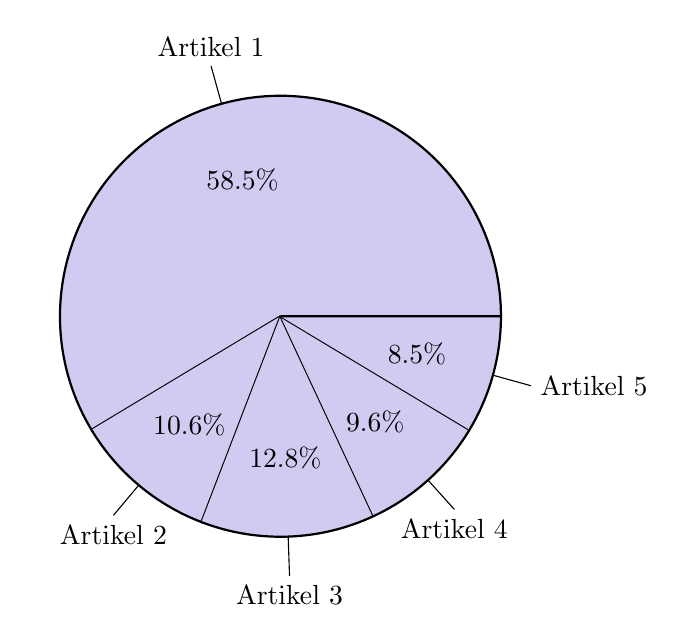
\begin{tikzpicture}
		\def\radius{2.8cm}
		\foreach \startA/\endA/\percent/\anchor/\name in {%
			0/211/58.5/above/Artikel 1,
			211/249/10.6/below/Artikel 2,
			249/295/12.8/below/Artikel 3,
			295/329/9.6/below/Artikel 4,
			329/360/8.5/right/Artikel 5}%
		{
			\draw[fill=mycolor, thick] (0,0) -- (\endA:\radius) arc (\endA:\startA:\radius)  node at ({0.5*\startA+0.5*\endA}:1.8cm) {\textcolor{black}{\percent \%}};
			\draw ({0.5*\startA+0.5*\endA}:\radius) -- ({0.5*\startA+0.5*\endA}:{\radius+0.5cm}) node[\anchor] {\textcolor{black}{\name}};
		};
	\end{tikzpicture}
\end{frame}



%----------------------------------------------------------%
 \begin{frame}
	\frametitle{Balkendiagramm}
	\begin{center}
	\begin{tikzpicture}
			\foreach \y in {-1,0,1,2,3,4}
				\draw[gray!50, text=black] (-2,\y cm) -- (6,\y cm);
 			%
 				\node[draw, rectangle, thick, minimum height=6cm, minimum width=1cm, fill=blue!20] at (-1, 1.5) {100 \%};
			\node[draw, rectangle, thick, minimum height=5.6cm, minimum width=1cm, fill=darkgreen!20] at (2, 1.3) {97.5 \%};
			\node[draw, rectangle, thick, minimum height=4.6cm, minimum width=1cm, fill=red!20] at (5, 0.8) {82.9 \%};
			%
			\node at (-1, 4.7) {187750};
			\node at (2, 4.3) {183150};
			\node at (5, 3.3) {155832};
			%
			\draw[thick] (-2,-1.5) -- (6,-1.5);
			\node at (-1,-2) {Zufällig};
			\node at (2,-2) {Algorithmus}; \node at (2,-2.4) {ohne Verbindung};
			\node at (5,-2) {Algorithmus}; \node at (5,-2.4) {mit Verbindung};
	\end{tikzpicture}
	\end{center}
\end{frame}



%----------------------------------------------------------%
\begin{frame}[fragile]
	\frametitle{Gestapeltes Balkendiagramm}
	\pgfplotstableread{
			Criterion      $Fahrt_1Klasse_1$     $Fahrt_2Klasse_1$    $Fahrt_3Klasse_1$    $Fahrt_4Klasse_2$
			Diff:+200        0   200   100     0   
			Diff:-100        50    0     0     0    
			Diff:-100        0     0     0   150     
		}\DatenStartVerteilung
	\begin{center}
			\begin{tikzpicture}
				  \begin{axis}[ybar=0pt,
				    ybar stacked,bar shift=0pt,
				    xticklabels from table={\DatenStartVerteilung}{Criterion},
				    xtick=data,
				    legend style={at={(1.025,1.0)},anchor=north west},
				    xlabel=Endergebnis]
				    \pgfplotstableforeachcolumn\DatenStartVerteilung\as\col{
				        \ifnum\pgfplotstablecol=0 
				        \else
				        \edef\tmp{
				            \noexpand\addplot table [x expr=\noexpand\coordindex,y=\col] {\noexpand\DatenStartVerteilung};
				            \noexpand\addlegendentry {\col}
				        }
				        \tmp
				        \fi}
				  \end{axis}
			\end{tikzpicture}
	\end{center}
\end{frame}



%----------------------------------------------------------%
\begin{frame}
	\frametitle{Graphen plotten}
	\begin{tikzpicture}[scale=0.8]
		\pgfplotsset{every axis legend/.style={rounded corners=2.5pt,inner xsep=3pt,inner ysep=2pt, draw=black!50,fill=white, font=\footnotesize,
			cells={anchor=center}, nodes={inner sep=2pt,text depth=0.15em,rounded corners=0pt,right},at={(1.05,0.5)}, anchor=west}}
		\begin{axis}[xmajorgrids, ymajorgrids, width=0.9\textwidth, height=0.9\textheight,
			y tick label style={/pgf/number format/1000 sep=.}, xlabel={Toleranz}, ylabel={Weglänge im Lager}]
			
			\addplot plot coordinates {
				(1, 1.83150)
				(2, 1.83150)
				(5, 1.83150)
				(8, 1.83150)
				(10, 1.83150)
				(15, 1.83150)
				(20, 1.83150)
 			};
 			\addlegendentry{keine Gewichtung}
			
		\addplot plot coordinates {
			(1, 1.83952)
			(2, 1.80658)
			(5, 1.70212)
			(8, 1.65560)
			(10, 1.64888)
			(15, 1.63770)
			(20, 1.63770)
 			};
 			\addlegendentry{Gewichtungsfaktor = 0,5}
 			
 			\addplot plot coordinates {
			(1, 1.83952)
			(2, 1.81538)
			(5, 1.67426)
			(8, 1.63136)
			(10, 1.63262)
			(15, 1.60042)
			(20, 1.60042)
 			};
 			\addlegendentry{Gewichtungsfaktor = 1}
 			
 			\addplot[thick, darkgreen, domain=0:20, samples=500]{0.1*sin(deg(x))+1.7};
 			\addlegendentry{Sinusfunktion}

			\end{axis}
	\end{tikzpicture}
\end{frame}



%----------------------------------------------------------%
\begin{frame}[c]
	\frametitle{Ausblick}
	\begin{itemize} 
		\item 3D berücksichtigen
		\item unterschiedliche Artikelgröße berücksichtigen
	\end{itemize}	
	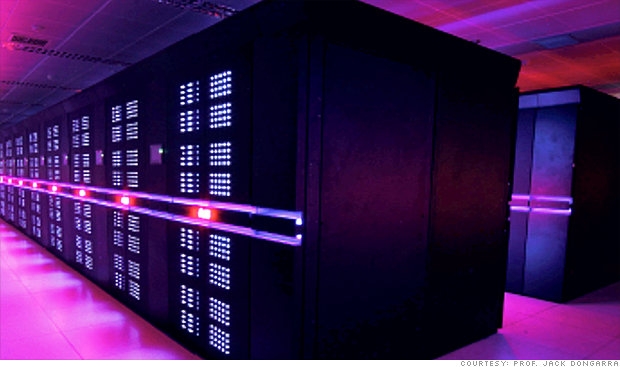
\includegraphics[trim=0pt 0pt 0pt 0pt, clip, width=0.7\textwidth]{../figs/z_supercomputer}
\end{frame}


%----------------------------------------------------------%
\begin{frame}[c]
	%\frametitle{Ausblick}
	\centering \bfseries Vielen Dank für Ihre Aufmerksamkeit!
	\\[15mm]
	
\includegraphics[trim=0pt 0pt 0pt 0pt, clip, width=0.45\textwidth]{../figs/z_jtl}
\end{frame}


\end{document}
% ---------------------------------------------------------------------------------















